\newcommand{\PP}{\mathbb{P}}
\newcommand{\EE}{\mathbb{E}}
\newcommand{\One}{\mathds{1}}
\makeatletter
\newcommand*{\rom}[1]{\expandafter\@slowromancap\romannumeral #1@}
\makeatother

%\newcommand{\R}{\mathbb{R}}
\newcommand{\B}{\mathcal{B}}
\newcommand{\eqnref}[1]{(\ref{eqn:#1})}
\newcommand{\figref}[1]{Figure~\ref{fig:#1}}
\newcommand{\prox}{\textrm{prox}}

\section{Introduction}

\begin{frame}{Introduction}

	Problem: $\min_{x \in \R^d} \frac{1}{n} \sum_{i=1}^n f_i(x) + h(x)$

	\begin{block}{SAGA}

	Given a learning rate $\gamma$, the value of $x^k$ and of each $f_i'
	(\phi_i^k)$ at the end of iteration $k$, it makes the following updates for
	iteration $k+1$:
	\begin{enumerate}
	\item Pick a $j$ uniformly at random.
	\item Take $\phi_j^{k+1} = x^k$, and store $f_j'(\phi_j^{k+1})$ in the table.
	\item Update $x$:
		\begin{equation*}
		w^{k+1} = x^k - \gamma \left[ f_j'(\phi_j^{k+1}) - f_j'(\phi_j^k)
		+ \frac1n \sum_{i=1}^n f_i'(\phi_i^k) \right] ,
		\end{equation*}
		$$x^{k+1} = \prox_\gamma^h (w^{k+1}).$$
	\end{enumerate}
	\end{block}

\end{frame}


\begin{frame}{Improvements}
	\vspace{2cm}
		\begin{itemize}
			\item Memory-efficiency $\rightarrow$ mini-batch SAGA
			\item Time-efficiency $\rightarrow$ distributed SAGA
		\end{itemize}
\end{frame}

\section{Mini-batch SAGA}

\begin{frame}{Mini-batch SAGA}

\begin{enumerate}
\item Pick a $i$ uniformly at random in $[1, \frac{n}m]$.
\item Take $\phi_j^{k+1} = x^k \ \forall \ j \in \B_i$, and store $\frac1m
	\sum_{j\in\B_i} f_j'(\phi_j^{k+1})$ in the table.
\item Update $x$:
\end{enumerate}

	\begin{equation*}
	w^{k+1} = x^k - \gamma \left[ \frac1m \sum_{j\in\B_i} f_j'(\phi_j^{k+1})
	- \frac1m \sum_{j\in\B_i} f_j'(\phi_j^k)
	+ \frac1n \sum_{i=1}^m \sum_{j\in\B_i} f_j'(\phi_j^k) \right] ,
	\end{equation*}
	$$x^{k+1} = \prox_\gamma^h (w^{k+1}).$$

\end{frame}

\begin{frame}{Results}

\begin{figure}[ht]
	\centering
	\subfigure{
		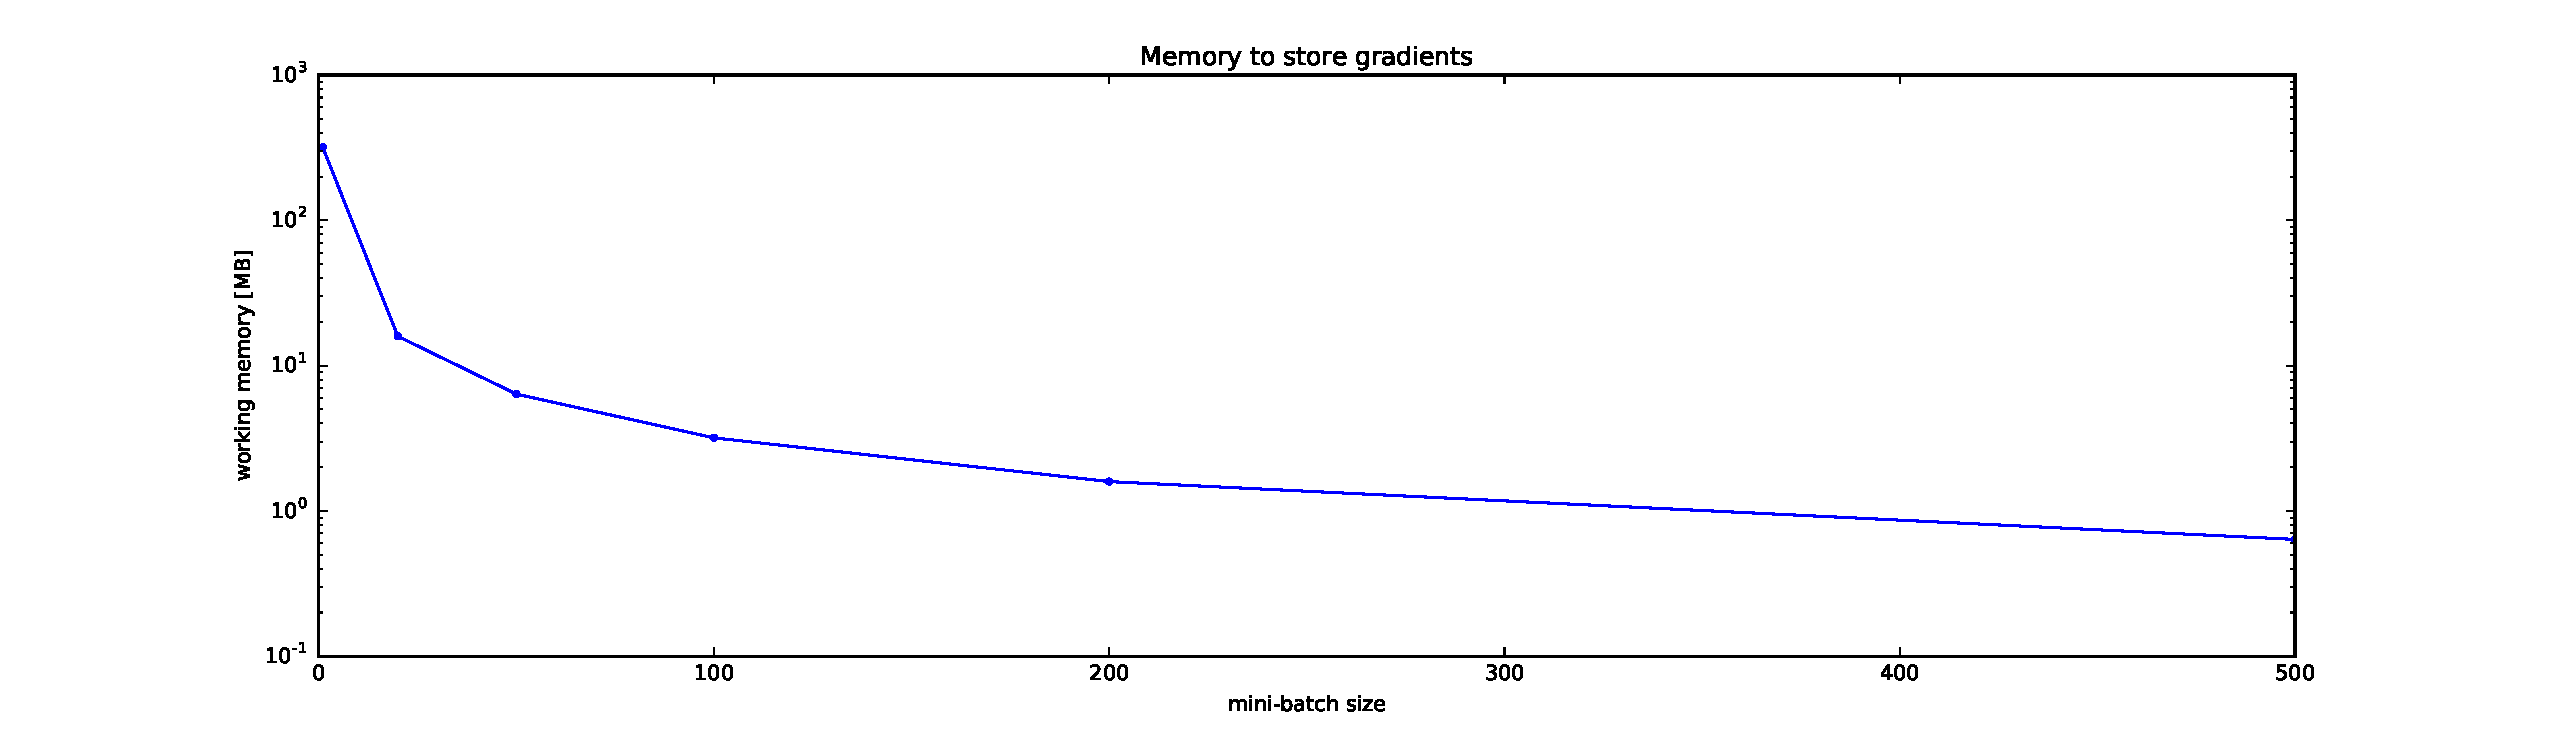
\includegraphics[height=3cm,width=0.45\columnwidth]{memory}}
	\hspace{0pt}
	\subfigure{
		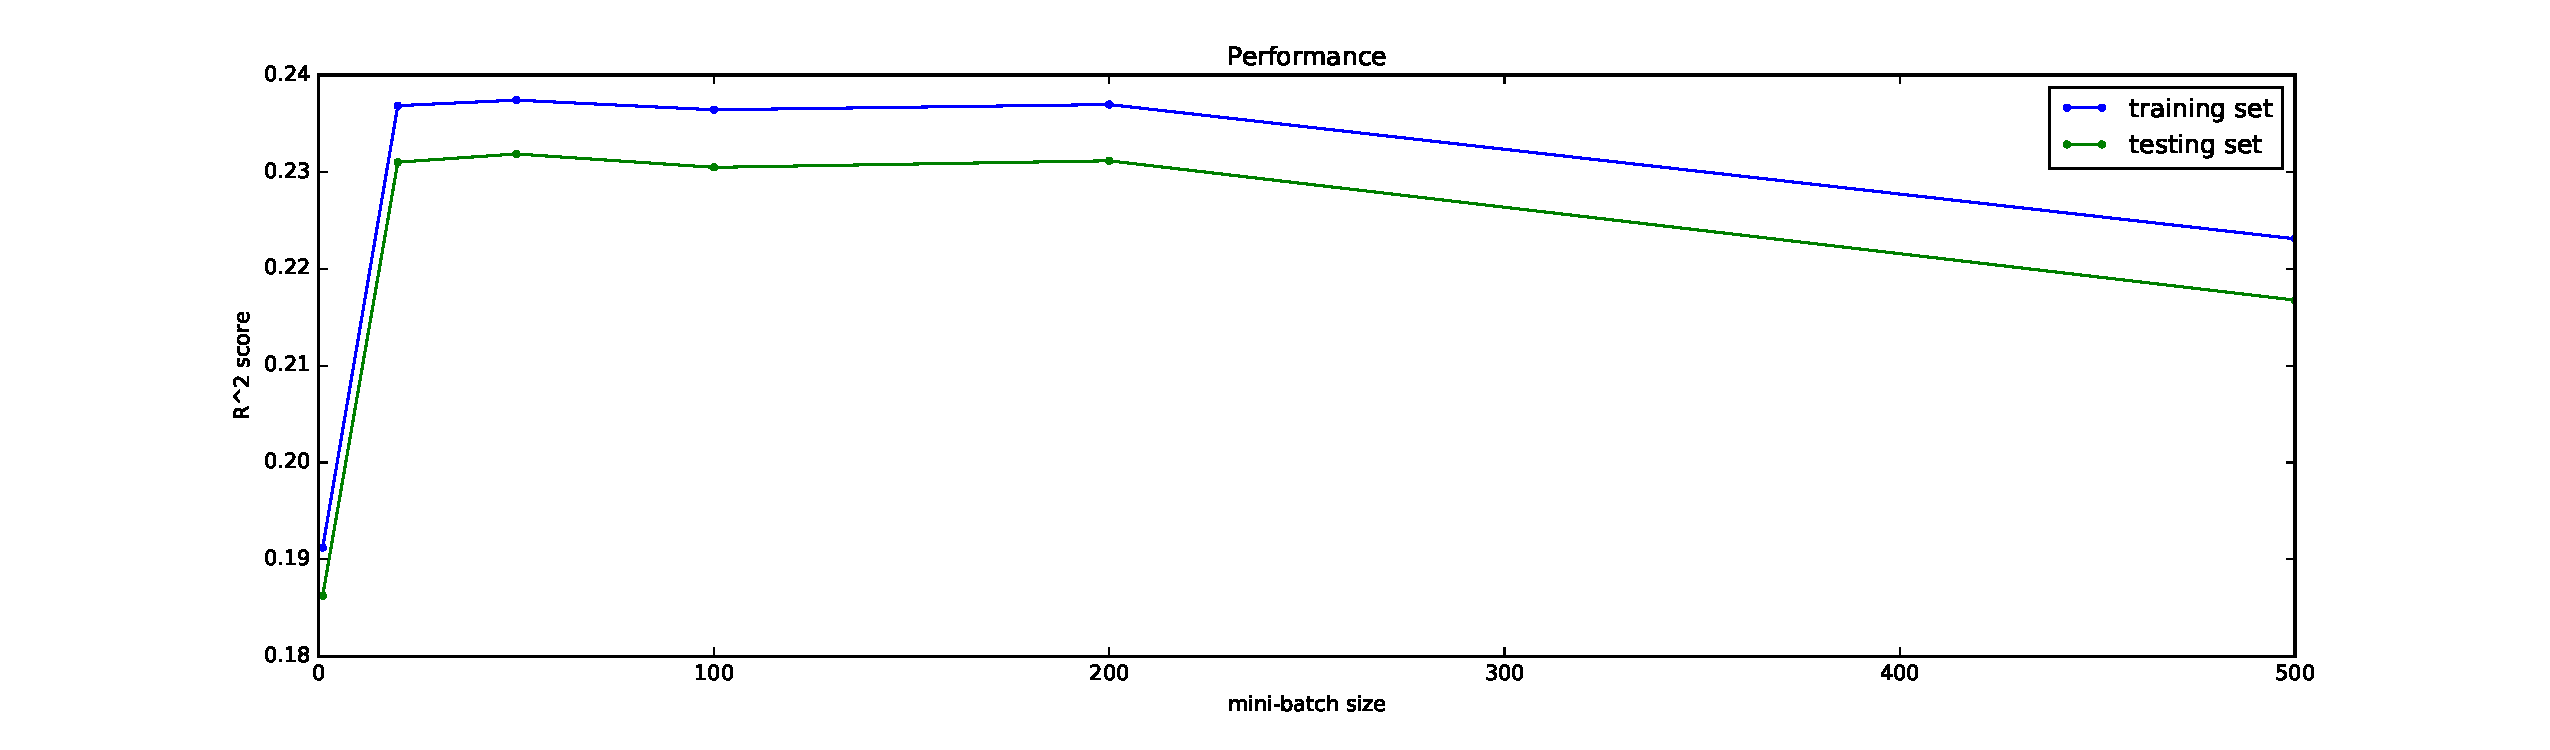
\includegraphics[height=3cm,width=0.45\columnwidth]{r2_score}}
	\\
	\subfigure{
		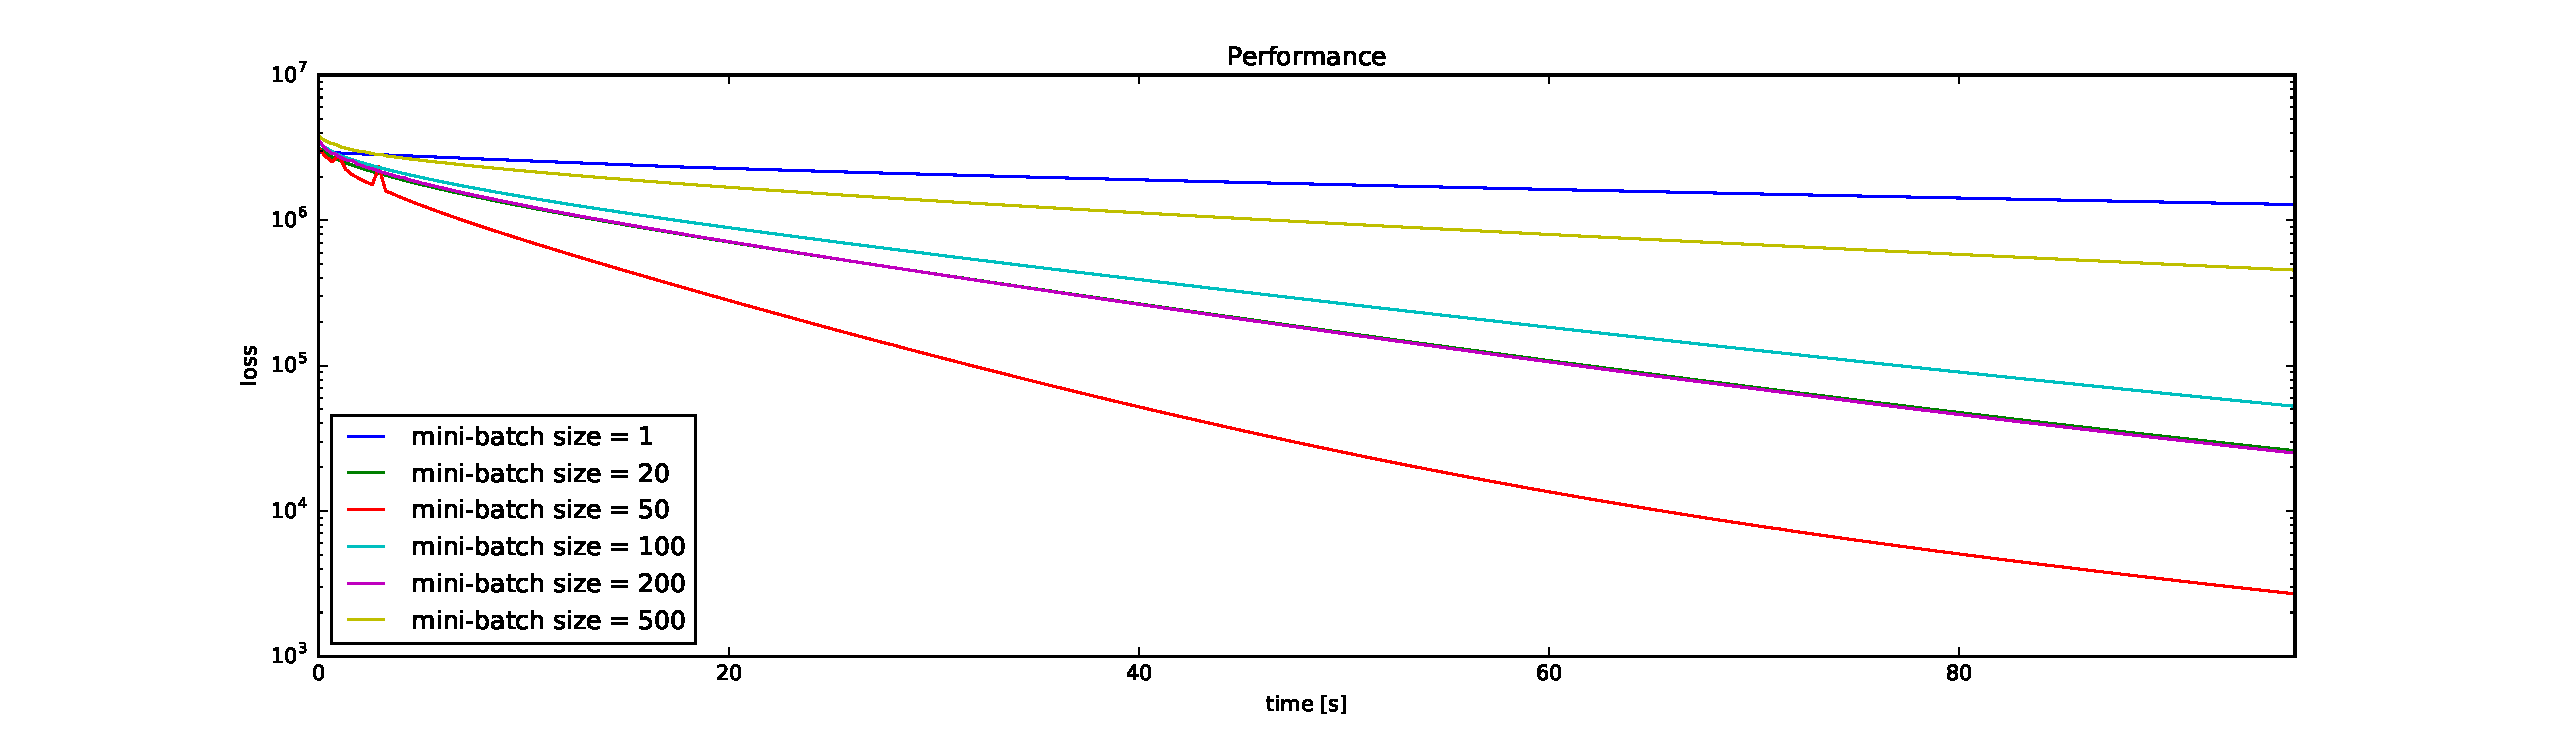
\includegraphics[height=4cm,width=0.7\columnwidth]{perf}}
	\caption{Performance evaluation of mini-batch SAGA.}
	\label{eval_saga_mb}
\end{figure}

\end{frame}

\section{Distributed SAGA}

\begin{frame}{The First Approach}
	\centering
	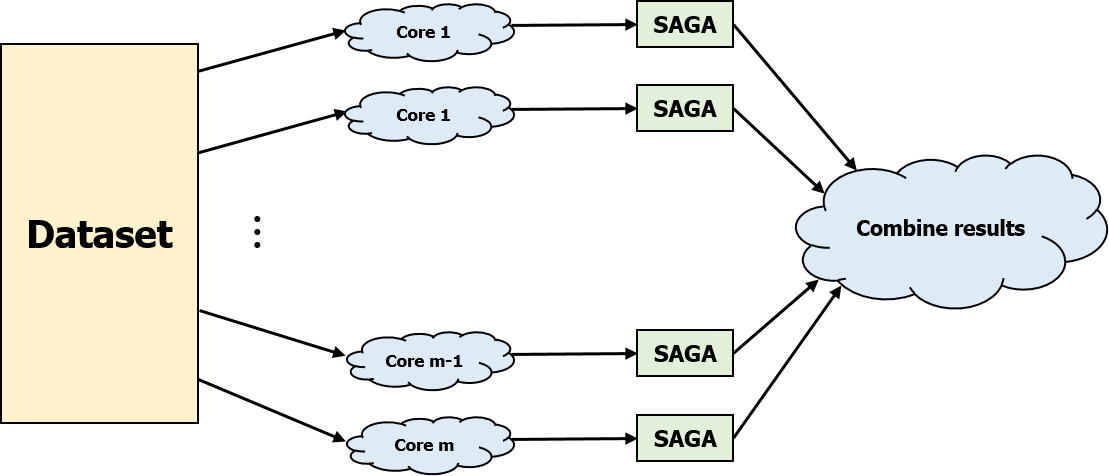
\includegraphics[scale=0.35]{Picture1.png}
	\visible<2>
	{
		\medskip
		\medskip
		\centering
		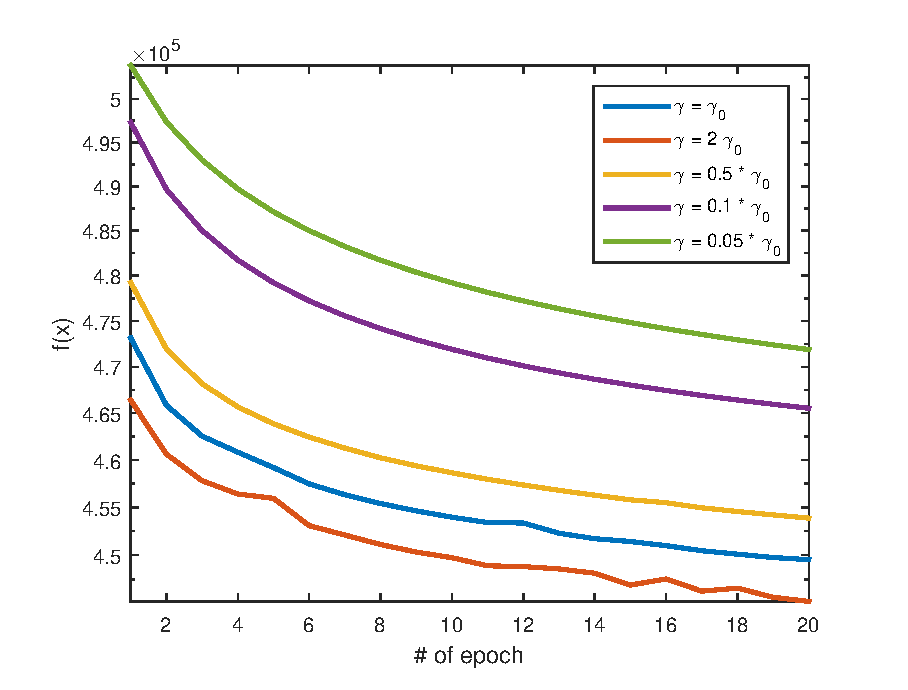
\includegraphics[scale=0.5]{distributed1.eps} 
	}
\end{frame}

\begin{frame}{The Second Approach}
	\centering
	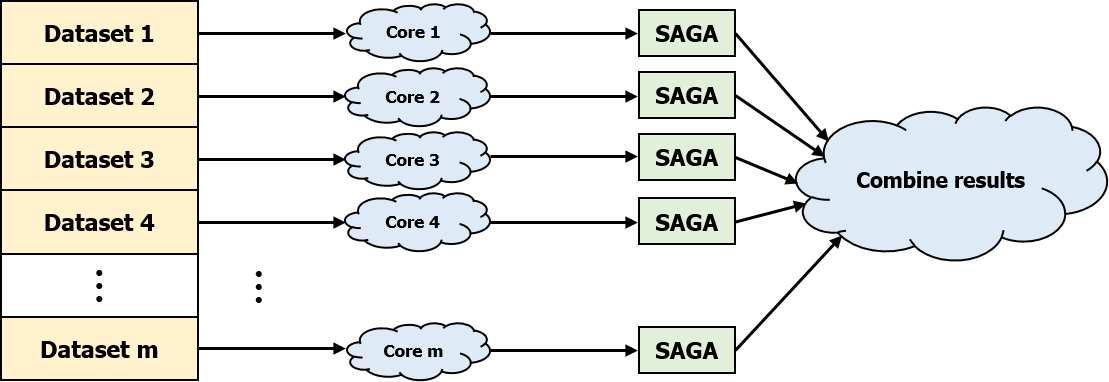
\includegraphics[scale=0.35]{Picture2.png}
	\visible<2->
	{
		\medskip
		\medskip
		\centering
		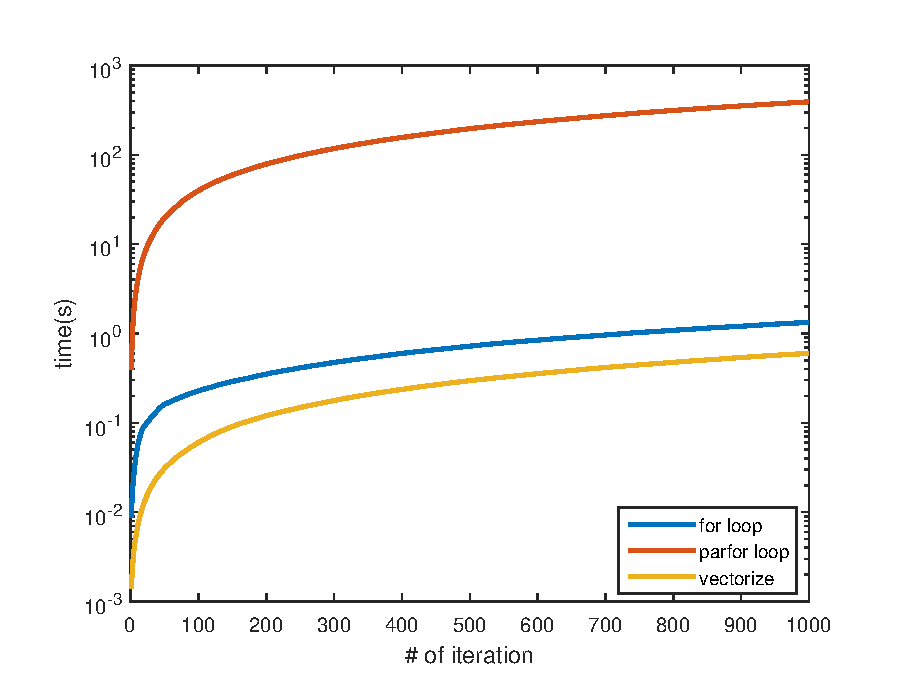
\includegraphics[scale=0.5]{distributed2.eps} 
	}
\end{frame}

\begin{frame}{The Second Approach}
	\centering
	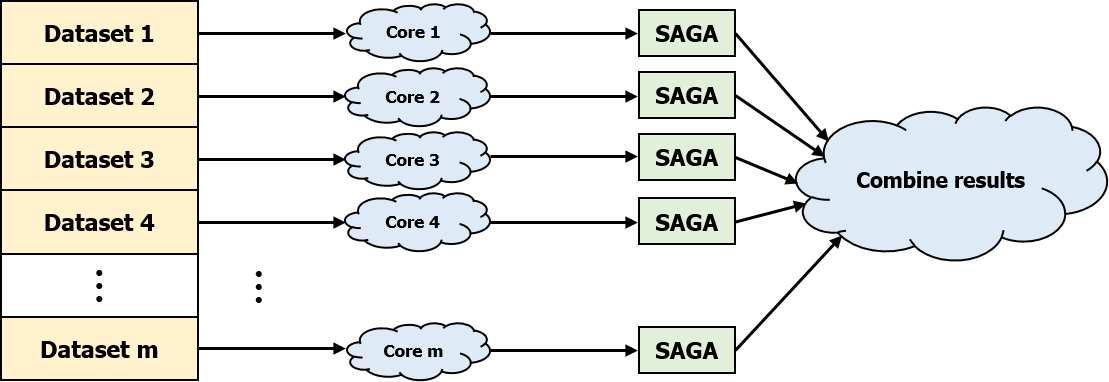
\includegraphics[scale=0.35]{Picture2.png}
	
	\centering
	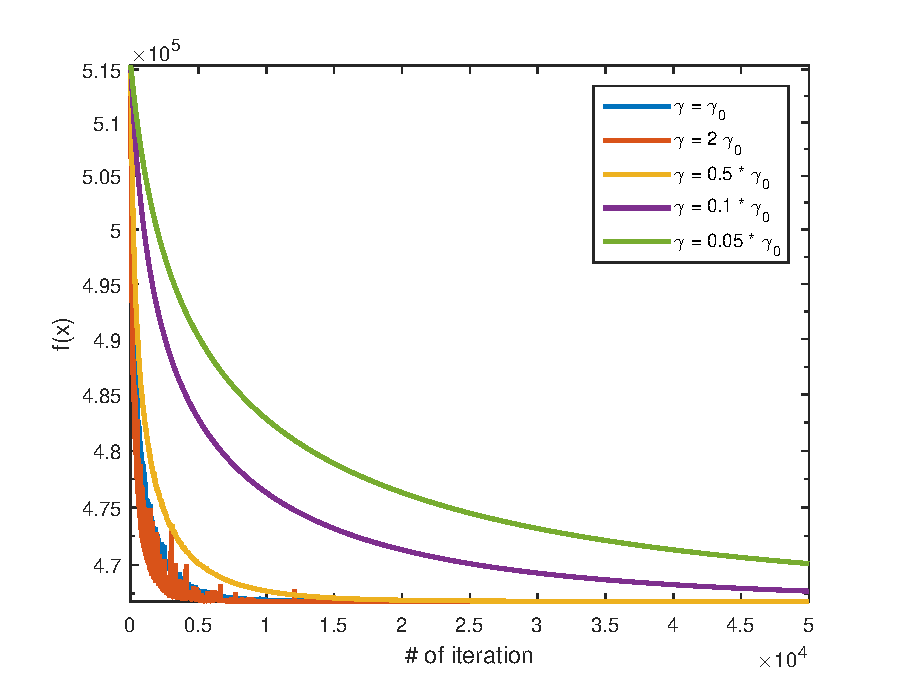
\includegraphics[scale=0.5]{distributed3.eps} 
\end{frame}

\begin{frame}{Compare First and Second Approach}
	\medskip
	\medskip
	\medskip
	\medskip
	\medskip
	\medskip
	\medskip
	\centering
	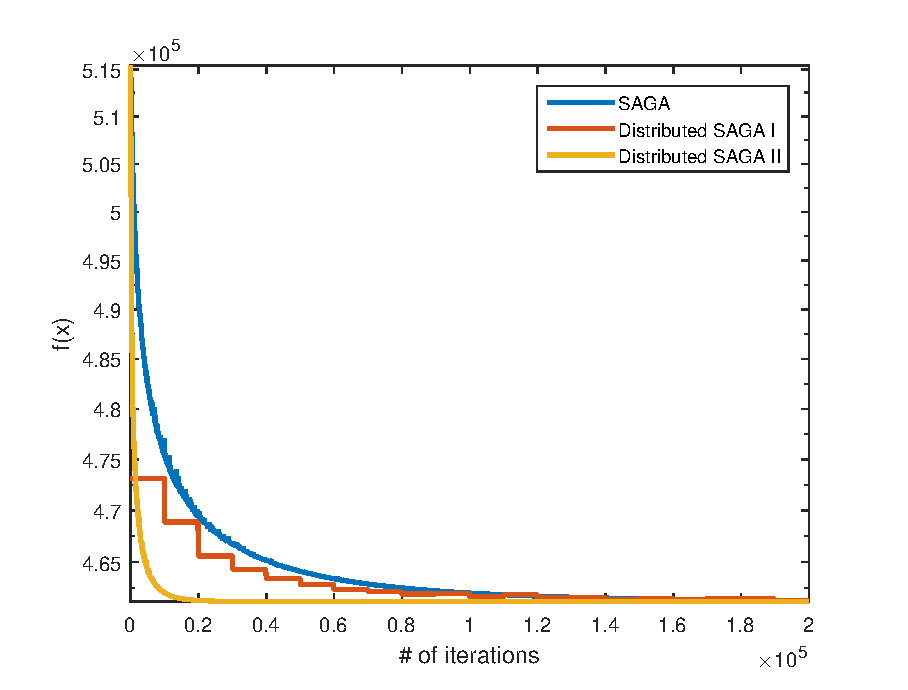
\includegraphics[scale=0.4]{compare.eps}
	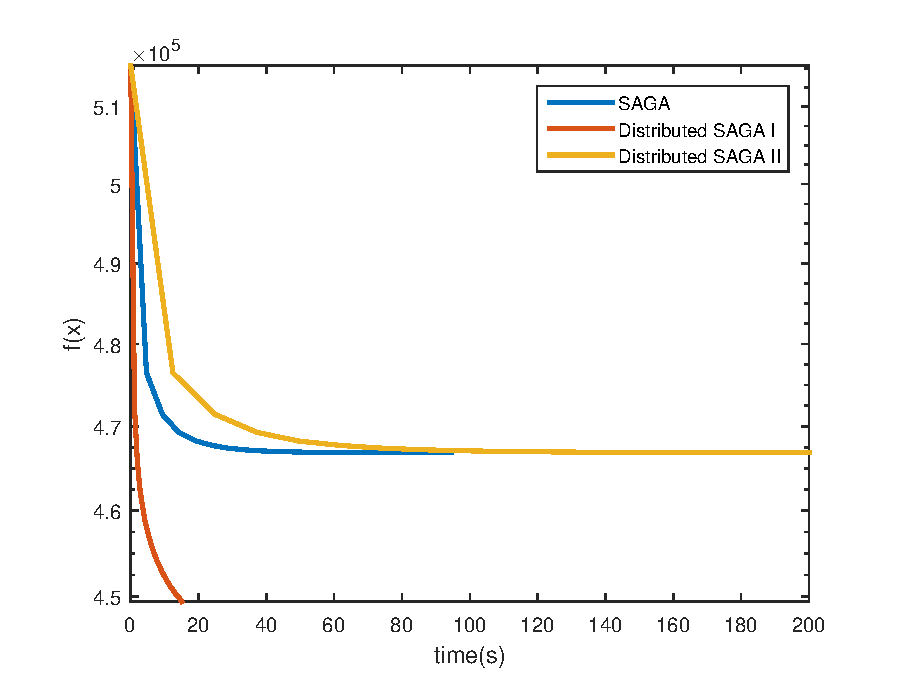
\includegraphics[scale=0.4]{compare2.eps} 
\end{frame}
